\section{Deskripsi Persoalan}
\subsection{Latar Belakang}
Pembatalan pemesanan merupakan persoalan nyata dalam industri perhotelan. Kamar yang telah dipesan lalu dibatalkan mendekati tanggal kedatangan berpotensi kosong, sementara penjualan ulang kamar yang diperkirakan batal berisiko menimbulkan \textit{overbooking} apabila tamu ternyata tetap datang. Dalam skenario tugas ini, Ronaldo Hotel\texttrademark{} membutuhkan sistem cerdas berbasis pembelajaran mesin klasik untuk memperkirakan pemesanan yang akan dibatalkan, tanpa sumber daya komputasi besar seperti \textit{deep learning}.

Persoalan ini dimodelkan sebagai klasifikasi biner. Setiap pemesanan direpresentasikan oleh atribut seperti jumlah tamu, lama menginap, jarak hari pemesanan terhadap kedatangan, tarif, dan kanal pemesanan. Target \texttt{is\_canceled} bernilai 1 apabila pemesanan dibatalkan dan 0 apabila tidak.

\subsection{Rumusan Persoalan dan Tujuan}
Kelompok diminta mengimplementasikan lima algoritma \textit{supervised learning} secara \textit{from scratch}, yaitu KNN, DTL, \textit{logistic regression}, SVM, dan \textit{Naive Bayes}. Implementasi tersebut dibandingkan dengan pustaka \textit{scikit-learn}, harus dapat disimpan dan dimuat ulang, serta digunakan untuk minimal satu \textit{submission} Kaggle yang \textit{reproducible}. Tahap pengolahan data mencakup \textit{data cleaning}, \textit{data transformation}, \textit{feature selection}, \textit{dimensionality reduction}, serta \textit{modeling and validation}. \textit{Preprocessing} pada data latih dan data uji dilakukan terpisah, dan kedua data tidak boleh digabungkan.

Tujuan laporan ini adalah menjelaskan pemahaman terhadap dataset, langkah \textit{cleaning} dan \textit{preprocessing} beserta alasannya, implementasi setiap algoritma, serta hasil eksperimen dan perbandingannya. Selain itu, laporan ini membahas visualisasi pohon keputusan, video lintasan parameter \textit{logistic regression}, visualisasi bidang pemisah SVM, graf \textit{Naive Bayes}, algoritma optimasi model, dan \textit{cost-sensitive classification}.

\subsection{Deskripsi Dataset}
Dataset terdiri atas \path{train.csv} dengan 27.373 baris berlabel dan \path{test.csv} dengan 6.844 baris tanpa label. Selain kolom \texttt{id} dan target, terdapat 17 fitur: 14 fitur numerik dan 3 fitur kategorikal. Kolom \texttt{id} hanya berfungsi sebagai pengenal baris pada berkas pengumpulan dan tidak digunakan sebagai fitur. Tabel~\ref{tab:fitur} merangkum fitur tersebut beserta proporsi nilai hilang pada data latih.

\begin{table}[htbp]
    \centering
    \small
    \renewcommand{\arraystretch}{1.08}
    \begin{tabularx}{\textwidth}{@{}l l r X@{}}
        \toprule
        Fitur & Tipe & Hilang (\%) & Keterangan \\
        \midrule
        \texttt{num\_adults} & numerik & 2,96 & Jumlah tamu dewasa (0--4). \\
        \texttt{num\_children} & numerik & 11,09 & Jumlah anak (0--10). \\
        \texttt{weekend\_nights} & numerik & 0 & Jumlah malam akhir pekan. \\
        \texttt{weekday\_nights} & numerik & 0 & Jumlah malam hari kerja. \\
        \texttt{meal\_package} & kategorikal & 6,43 & Paket makan: Breakfast, Room Only, Half Board, Full Board. \\
        \texttt{needs\_parking} & numerik & 3,95 & Kebutuhan parkir (0/1). \\
        \texttt{room\_category} & kategorikal & 3,66 & Tipe kamar A--G. \\
        \texttt{days\_before\_arrival} & numerik & 4,10 & Selisih hari pemesanan dan kedatangan (0--448). \\
        \texttt{arrival\_year} & numerik & 0 & Tahun kedatangan (2023 atau 2024). \\
        \texttt{arrival\_month} & numerik & 0 & Bulan kedatangan. \\
        \texttt{arrival\_day} & numerik & 0 & Tanggal kedatangan. \\
        \texttt{booking\_channel} & kategorikal & 0 & Kanal: Online Travel Agent, Offline Agent, Corporate, Complimentary, Airline. \\
        \texttt{is\_returning\_guest} & numerik & 0 & Tamu yang pernah menginap (0/1). \\
        \texttt{prior\_cancellations} & numerik & 0 & Jumlah pembatalan sebelumnya. \\
        \texttt{prior\_completed\_bookings} & numerik & 0 & Jumlah pemesanan sebelumnya yang tidak dibatalkan. \\
        \texttt{nightly\_rate\_idr} & numerik & 7,45 & Tarif per malam dalam rupiah. \\
        \texttt{special\_requests} & numerik & 9,13 & Jumlah permintaan khusus (0--5). \\
        \bottomrule
    \end{tabularx}
    \caption{Fitur dataset dan proporsi nilai hilang pada \texttt{train.csv}.}
    \label{tab:fitur}
\end{table}

\subsection{Pemahaman Data}\label{sec:eda}
Pemahaman data dimulai dari distribusi kelas. Sebanyak 32,77\% pemesanan pada data latih berlabel batal. Dataset tidak seimbang secara ekstrem, tetapi tebakan yang selalu memilih kelas mayoritas sudah memperoleh akurasi 0,6723 pada data validasi. Angka ini menjadi baseline yang harus dilampaui setiap model.

Dari sisi kualitas data, delapan fitur memiliki nilai hilang, dan 10.737 baris latih memiliki sedikitnya satu nilai hilang. Karena jumlah tersebut mencapai 39\% data latih, penghapusan baris akan membuang terlalu banyak informasi sehingga imputasi atau penanganan nilai hilang di dalam model lebih tepat. Pemeriksaan pada seluruh \path{train.csv} juga menemukan 66 salinan duplikat berdasarkan fitur, dua kelompok duplikat dengan label bertentangan, dan 64 baris tanpa malam menginap. Tidak ada baris tanpa tamu. Aturan IQR menandai cukup banyak pencilan, misalnya 916 baris pada \texttt{days\_before\_arrival} dan 1.144 baris pada \texttt{nightly\_rate\_idr}.

Hubungan fitur dengan target terlihat dari korelasi. Korelasi linear terkuat terhadap target dimiliki \texttt{days\_before\_arrival} ($+0{,}440$) dan \texttt{special\_requests} ($-0{,}258$), diikuti \texttt{arrival\_year} ($+0{,}180$) dan \texttt{nightly\_rate\_idr} ($+0{,}134$). Artinya, pemesanan yang dibuat jauh hari sebelum kedatangan lebih sering dibatalkan, sedangkan tamu yang mengajukan permintaan khusus cenderung datang. Gambar~\ref{fig:eda-kategori} menunjukkan rasio pembatalan per kategori. Kanal Corporate dan Complimentary jauh lebih jarang batal dibanding rata-rata, sedangkan paket Half Board dan kamar Type A lebih sering batal.

\begin{figure}[htbp]
    \centering
    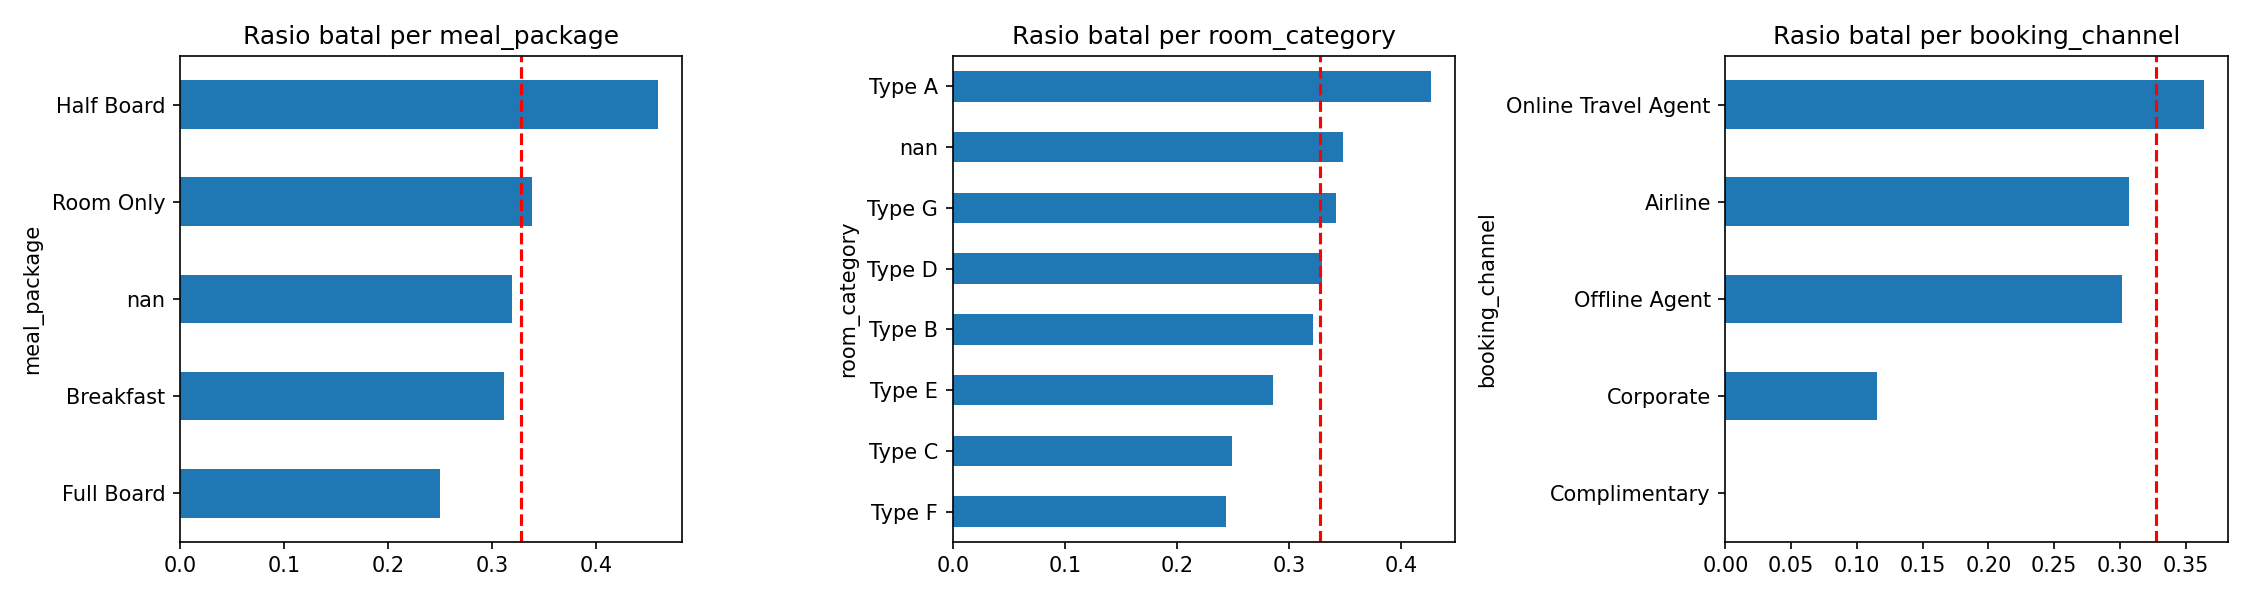
\includegraphics[width=\textwidth]{output/eda/cancel_rate_categorical.png}
    \caption{Rasio pembatalan per kategori. Garis merah menandai rasio pembatalan keseluruhan.}
    \label{fig:eda-kategori}
\end{figure}

\begin{figure}[htbp]
    \centering
    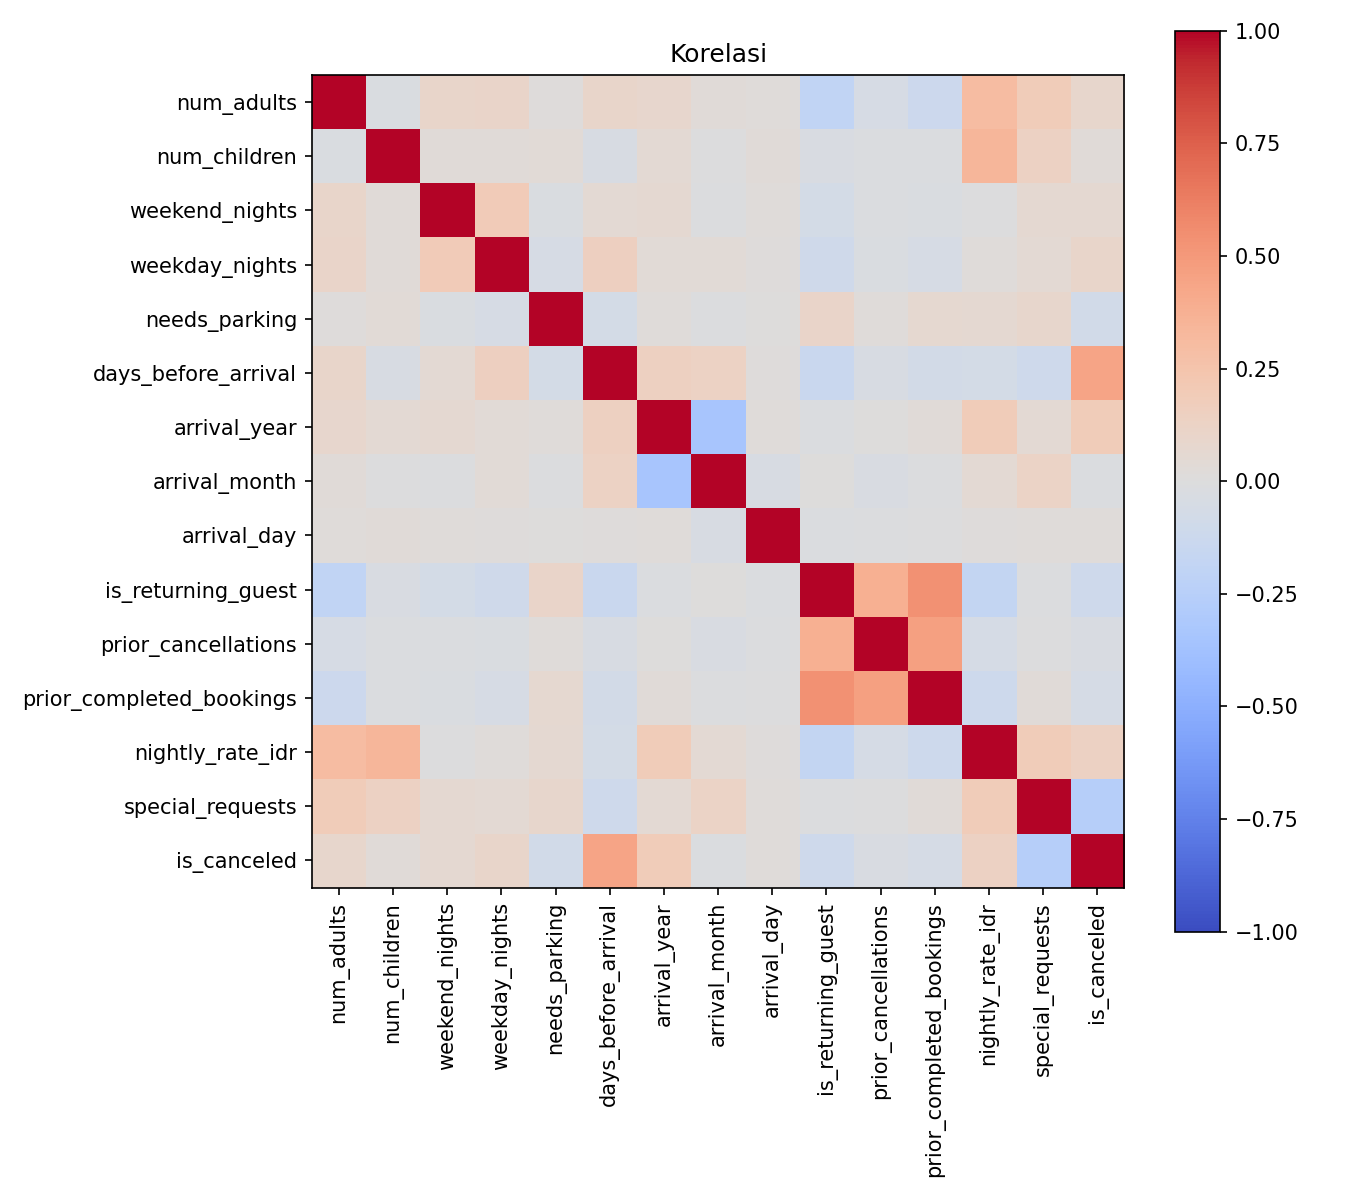
\includegraphics[width=0.72\textwidth]{output/eda/correlation.png}
    \caption{Matriks korelasi Pearson antarfitur numerik dan target.}
    \label{fig:eda-korelasi}
\end{figure}

Data latih dan data uji juga dibandingkan untuk mendeteksi pergeseran distribusi. Statistik Kolmogorov--Smirnov untuk fitur numerik dan \textit{total variation distance} untuk fitur kategorikal seluruhnya di bawah 0,015. Proporsi nilai hilang pada data uji juga mendekati data latih, misalnya 10,91\% berbanding 11,09\% untuk \texttt{num\_children}, dan tidak ada kategori baru pada data uji. Dengan demikian, distribusi data uji dapat dianggap sama dengan data latih, sehingga skor validasi lokal dapat digunakan sebagai perkiraan kinerja pada Kaggle. Pemeriksaan ini hanya membandingkan distribusi fitur dan tidak menggunakan label uji.
